\section{\texorpdfstring{$\mathcal{V}$}{V} 算子}\label{sec:vanishing-set-operator}

为了研究多项式的零点集, 首先要明确这些多项式及其解分别属于哪里. 选定一个域 $K$, 称为\textbf{基域}, 并考虑多项式环 $K[x_{1},\ldots,x_{n}]$. 这个环的元素除了可视为抽象的多项式之外, 还可用来定义以 $K^{n}$ 的元素为输入, 以 $K$ 的元素为输出的函数. 例如, 多项式
\[
  f=2xy+4z^{2}\in\mathbb{R}[x,y,z]
\]
定义了一个从 $\mathbb{R}^{3}$ 到 $\mathbb{R}$ 的函数. 若输入元素 $(1,-1,3)$, 则 $f$ 的输出是一个实数:
\[
  f(1,-1,3)=2\cdot1\cdot(-1)+4\cdot3^{2}=34.
\]
多项式函数的定义域称为仿射空间.

\begin{Definition}{仿射空间}\leavevmode\label{def:affine-space}
  $K$ 上的 $n$ 维\textbf{仿射空间}记作 $\mathbb{A}^{n}_{K}$, 是由 $K$ 中元素组成的 $n$ 元组的集合:
  \[
    \mathbb{A}^{n}_{K}=\{(a_{1},\ldots,a_{n})\mid a_{i}\in K\}.
  \]
\end{Definition}

\BookPairedNote
  {作为集合, $\mathbb{A}^{n}_{K}$ 与向量空间 $K^{n}$ 相同. 那么, 为什么要另起一个名字, 另用一个记号呢? 写成 $K^{n}$ 时, 我们把这个集合看成具有加法和数乘运算的代数对象, 也就是一个向量空间.}
  {$K^{n}$ 的元素通常称为\textquotedbl{}向量\textquotedbl{}, 而 $\mathbb{A}^{n}_{K}$ 的元素称为\textquotedbl{}点\textquotedbl{}, 以突出它们的几何意义.}
\noindent 相反, 写成 $\mathbb{A}^{n}_{K}$ 时, 我们不考虑这个集合的代数结构: 不再把它的元素看成可以相加的向量, 而把它们看成多项式函数的输入. 特别地, 元素 $(0,\ldots,0)$ 在向量空间 $K^{n}$ 中十分特殊, 因为它是加法单位元; 但在仿射空间 $\mathbb{A}^{n}_{K}$ 中, 它与任何其他元素并无实质区别.

\BookPairedNoteLeft
  {当基域 $K$ 可由上下文确定时, 我们通常只写 $\mathbb{A}^{n}$, 不写 $\mathbb{A}^{n}_{K}$.}
  {为了区分多项式与它们的取值, 我们用字母表末尾的字母 ($x$, $y$ 和 $z$) 表示变量, 用字母表开头的字母 ($a$, $b$ 和 $c$) 表示 $K$ 的元素.}
\noindent 例如, $f=x^{2}y$ 表示环 $K[x,y]$ 的一个元素, 而 $f(a,b)=a^{2}b$ 表示在点 $(a,b)\in\mathbb{A}^{2}$ 处对 $f$ 求值所得的 $K$ 的元素. 如果 $f\in K[x_{1},\ldots,x_{n}]$ 对某点 $(a_{1},\ldots,a_{n})\in\mathbb{A}^{n}$ 满足
\[
  f(a_{1},\ldots,a_{n})=0,
\]
就称 $f$ 在 $(a_{1},\ldots,a_{n})$ 处为零.

给定一个多项式 $f\in K[x_{1},\ldots,x_{n}]$, $f$ 取值为零的所有点组成的集合是 $\mathbb{A}^{n}$ 的一个子集. 例如, 若
\[
  f=y-x^{2}\in\mathbb{R}[x,y],
\]
\BookPairedFigure
  {则 $f$ 在点 $(0,0)$, $(1,1)$, $(2,4)$, $(-1,1)$ 等处取值为零. $\mathbb{A}^{2}_{\mathbb{R}}$ 中使 $f=y-x^{2}$ 为零的所有点组成了我们熟悉的抛物线. 这是我们第一次接触代数几何: 一个代数对象, 即环 $\mathbb{R}[x,y]$ 的元素 $y-x^{2}$, 引出了一个几何对象, 即这条抛物线.}
  {\phantomsection\label{fig:parabola-vanishing-set}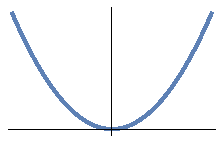
\includegraphics[width=\linewidth]{figures/parabola-1-1.pdf}}

更一般地, 对一个 (可能是无限的) 多项式集合, 可以研究 $\mathbb{A}^{n}$ 中使集合内每个多项式都为零的点所成的集合.

\begin{Definition}{零点集}\leavevmode\label{def:vanishing-set}
  设 $S\subseteq K[x_{1},\ldots,x_{n}]$ 是一个多项式集合. $S$ 的\textbf{零点集}为
  \[
    \mathcal{V}(S)=\{(a_{1},\ldots,a_{n})\in\mathbb{A}^{n}\mid
      f(a_{1},\ldots,a_{n})=0 \text{ 对所有 } f\in S\}\subseteq\mathbb{A}^{n}.
  \]
\end{Definition}

通常称 $\mathcal{V}(S)$ 中的点为 $S$ 中多项式的解. 当 $S=\{f_{1},\ldots,f_{r}\}$ 是有限集时, 我们写 $\mathcal{V}(f_{1},\ldots,f_{r})$, 而不写 $\mathcal{V}(\{f_{1},\ldots,f_{r}\})$.

\begin{Example}{$\mathbb{A}^{2}_{\mathbb{R}}$ 中的曲线}\leavevmode\label{ex:plane-curves}
  考虑 $S=\{y-x^{2}\}\subseteq K[x,y]$. 那么 $\mathcal{V}(S)=\{(a,a^{2})\mid a\in K\}\subseteq\mathbb{A}^{2}$. 当 $K=\mathbb{R}$ 时, 这就是\hyperref[fig:parabola-vanishing-set]{上面的抛物线}. 类似地, $\mathcal{V}(x^{2}+y^{2}-1)$, $\mathcal{V}(y^{2}-x^{3}-x^{2})$ 和 $\mathcal{V}(y^{2}-(x+1)^{3})$ 是\hyperref[fig:three-plane-curves]{下图}所示的 $\mathbb{A}^{2}_{\mathbb{R}}$ 中的平面曲线.
  \par\smallskip
  {\centering\phantomsection\label{fig:three-plane-curves}%
    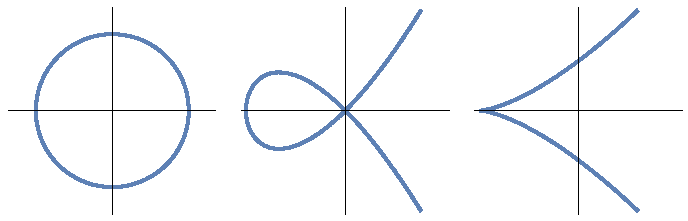
\includegraphics[width=.94\linewidth]{figures/plane-curves-1-3.pdf}\par}
\end{Example}

\begin{Example}{$\mathbb{A}^{3}_{\mathbb{R}}$ 中的曲面}\leavevmode\label{ex:three-surfaces}
  零点集 $\mathcal{V}(x^{2}+y^{2}+z^{2}-1)$, $\mathcal{V}(x^{2}+y^{2}-z^{2})$ 和 $\mathcal{V}(x^{2}+y^{2}z)$ 分别是单位球面, 圆锥面以及\textquotedbl{}Whitney 伞\textquotedbl{}, 如\hyperref[fig:sphere-cone-and-whitney-umbrella]{下图}在 $\mathbb{A}^{3}_{\mathbb{R}}$ 中所示.
  \par\smallskip
  {\centering\phantomsection\label{fig:sphere-cone-and-whitney-umbrella}%
    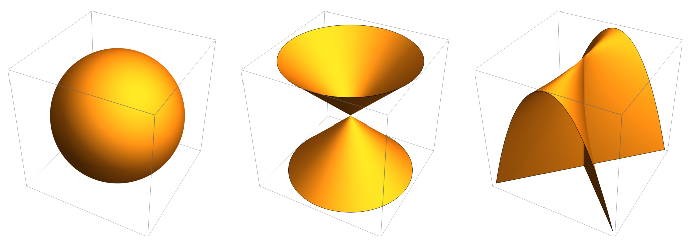
\includegraphics[width=.94\linewidth]{figures/surfaces-1-4.pdf}\par}
\end{Example}

\begin{Example}{坐标轴}\leavevmode\label{ex:vanishing-set-coordinate-axes}
  若 $S=\{xy\}\subseteq K[x,y]$, 则 $\mathcal{V}(S)=\{(a,b)\in\mathbb{A}^{2}\mid ab=0\}\subseteq\mathbb{A}^{2}$. 由于 $K$ 是域, $ab=0$ 当且仅当 $a=0$ 或 $b=0$ (或者两者都为零), 所以 $\mathcal{V}(S)$ 是满足 $a=0$ 的点与满足 $b=0$ 的点的并集. 当 $K=\mathbb{R}$ 时, 这就是实平面 $\mathbb{A}^{2}_{\mathbb{R}}$ 中的 $x$ 轴与 $y$ 轴的并集.
\end{Example}

\begin{Example}{单点}\leavevmode\label{ex:singleton-vanishing-sets}
  令 $S=\{x,y\}\subseteq K[x,y]$. 那么
  \[
    \mathcal{V}(S)=\{(a,b)\in\mathbb{A}^{2}\mid a=0\text{ 且 }b=0\}
      =\{(0,0)\}\subseteq\mathbb{A}^{2}.
  \]
  也就是说, $\mathcal{V}(S)$ 由一个点组成, 即原点.

  类似地, 若 $S=\{x-\mathrm{i},y-1-\mathrm{i},z-5\}\subseteq\mathbb{C}[x,y,z]$, 则
  \[
    \mathcal{V}(S)=\{(\mathrm{i},1+\mathrm{i},5)\}\subseteq\mathbb{A}^{3}_{\mathbb{C}},
  \]
  这同样是一个单点.
\end{Example}

\begin{Example}{$\mathbb{A}^{3}$ 中的一条曲线}\leavevmode\label{ex:space-curve-intersection}
  \BookPairedFigure
    {集合
     \[
       S=\{x^{2}+y^{2}-1,x^{2}-y^{2}-z\}
         \subseteq\mathbb{R}[x,y,z]
     \]
     的零点集由 $\mathbb{A}^{3}_{\mathbb{R}}$ 中使 $a^{2}+b^{2}-1$ 和 $a^{2}-b^{2}-c$ 都为零的点 $(a,b,c)$ 组成. \hyperref[fig:intersection-of-two-surfaces]{图中}将这条曲线画成两个曲面的交, 每个曲面对应一个定义它的多项式.}
    {\phantomsection\label{fig:intersection-of-two-surfaces}%
      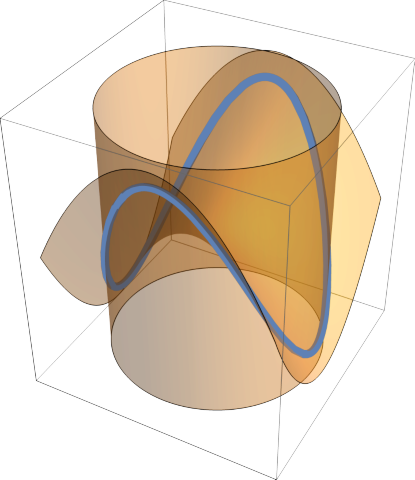
\includegraphics[width=.94\linewidth]{figures/intersection-curve-1-7.png}}
\end{Example}

\BookPairedNoteLeft
  {上面各图的基域都是 $K=\mathbb{R}$. 在 $\mathbb{R}$ 上, 我们有一定的几何直觉; 例如, 大致知道\textquotedbl{}曲线\textquotedbl{}或\textquotedbl{}曲面\textquotedbl{}意味着什么. 代数几何的目标是在一般的域上精确地表述这种直觉.}
  {既然现在把多项式看作函数 $\mathbb{A}^{n}\to K$, 就值得指出多项式与多项式函数之间有一个微妙却重要的区别. 尤其让人有些意外的是, $K[x_{1},\ldots,x_{n}]$ 中不同的多项式可以给出同一个函数 $\mathbb{A}^{n}\to K$.}

例如, 设 $K=\mathbb{F}_{2}=\{0,1\}$, 即含两个元素的域; 回顾一下, 这个域的加法与乘法都是模 $2$ 进行的. 令
\begin{equation}\label{eq:distinct-polynomials-over-two-elements}
  f(x)=1+x+x^{2} \qquad\text{以及}\qquad g(x)=1.
\end{equation}
作为 $\mathbb{F}_{2}[x]$ 的元素, 这两个多项式不相等, 因为它们在单项式 $x$ 和 $x^{2}$ 上的系数不同. 然而, 将它们视作函数 $\mathbb{A}^{1}\to\mathbb{F}_{2}$ 时, 可以看到
\[
  f(0)=1+0+0^{2}=1=g(0) \qquad\text{以及}\qquad
  f(1)=1+1+1^{2}=1=g(1).
\]
因此, 对定义域中的每一个输入, $f$ 和 $g$ 给出同一个输出. 所以尽管它们作为多项式不同, 作为函数却相等.

为了更一般地描述多项式与其对应函数的区别, 令 $K[\mathbb{A}^{n}]$ 表示多项式函数 $\mathbb{A}^{n}\to K$ 的集合. 也就是说, $K[\mathbb{A}^{n}]$ 的元素是形如
\[
  (a_{1},\ldots,a_{n})\mapsto f(a_{1},\ldots,a_{n})
\]
的函数, 其中 $f\in K[x_{1},\ldots,x_{n}]$. 稍加思考即可看出, $K[\mathbb{A}^{n}]$ 在取值于 $K$ 的函数加法与乘法下构成一个环. 把多项式送到其对应函数, 就定义了一个满的环同态 $K[x_{1},\ldots,x_{n}]\to K[\mathbb{A}^{n}]$. 恰好在不同的多项式给出同一个函数时, 这个同态不是单射. 例如,
\[
  \mathbb{F}_{2}[x]\to\mathbb{F}_{2}[\mathbb{A}^{1}]
\]
不是单射, 因为 \eqref{eq:distinct-polynomials-over-two-elements} 中定义的不同多项式 $f,g\in\mathbb{F}_{2}[x]$ 在 $\mathbb{F}_{2}[\mathbb{A}^{1}]$ 中给出同一个多项式函数.

下面的结果表明, 上述现象仅在有限域中出现, 因而只要假定 $K$ 是无限域, 就不必担心这一细微差别.

\begin{Proposition}{多项式与函数}\leavevmode\label{prop:polynomial-function-isomorphism}
  将多项式送到对应函数的环同态 $K[x_{1},\ldots,x_{n}]\to K[\mathbb{A}^{n}]$ 是同构, 当且仅当 $K$ 是无限域.
\end{Proposition}

\begin{Proof}
  我们证明这个充要条件的两个方向.

  ($\Rightarrow$) 用逆否命题来证明. 假设 $K=\{a_{1},\ldots,a_{n}\}$ 是有限域, 考虑非零多项式
  \[
    f=\prod_{i=1}^{n}(x_{1}-a_{i})\in K[x_{1}]\subseteq K[x_{1},\ldots,x_{n}].
  \]
  把 $K$ 中的任何值代入 $x_{1}$, 都会使一个因子为零. 所以 $f$ 定义了零函数 $\mathbb{A}^{n}\to K$. 这表明 $K[x_{1},\ldots,x_{n}]\to K[\mathbb{A}^{n}]$ 不是同构.

  ($\Leftarrow$) 假设 $K$ 是无限域. 根据定义, $K[x_{1},\ldots,x_{n}]\to K[\mathbb{A}^{n}]$ 是满射. 因此只需证明它是单射, 或者等价地, 证明它的核只含零多项式. 为此对 $n$ 作归纳.

  (归纳起点) 假设 $h\in K[x]$ 定义了零函数 $\mathbb{A}^{1}\to K$. 因为 $K$ 是无限域, 这意味着 $h$ 有无穷多个零点. 根据 Corollary~\ref{cor:polynomial-finite-zeros}, 非零多项式只有有限多个零点, 所以 $h$ 必为零多项式.

  (归纳步骤) 假设 $h\in K[x_{1},\ldots,x_{n}]$ 定义了零函数, 写成
  \[
    h=\sum_{i=0}^{d}h_{i}x_{n}^{i},
  \]
  其中 $h_{i}\in K[x_{1},\ldots,x_{n-1}]$. 对每个 $(a_{1},\ldots,a_{n-1})\in\mathbb{A}^{n-1}$, 一元多项式 $h(a_{1},\ldots,a_{n-1},x_{n})\in K[x_{n}]$ 定义了零函数 $\mathbb{A}^{1}\to K$. 因此, 按照归纳起点中的论证, $h(a_{1},\ldots,a_{n-1},x_{n})$ 是零多项式. 特别地, 对所有 $i$ 都有 $h_{i}(a_{1},\ldots,a_{n-1})=0$. 由于这对每个 $(a_{1},\ldots,a_{n-1})\in\mathbb{A}^{n-1}$ 都成立, 所以对所有 $i$, $h_{i}:\mathbb{A}^{n-1}\to K$ 都是零函数. 根据归纳假设, 对每个 $i$, $h_{i}\in K[x_{1},\ldots,x_{n-1}]$ 都是零多项式, 从而 $h$ 是零多项式.
\end{Proof}

\BookExerciseHeading
\begin{BookExercises}
  \item\label{ex:sketch-vanishing-sets} 画出下列零点集的草图.
    \begin{enumerate}[label=(\alph*)]
      \item $\mathcal{V}(x^{2}-1)\subseteq\mathbb{A}^{1}_{\mathbb{R}}$
      \item $\mathcal{V}(x^{2}-y^{2})\subseteq\mathbb{A}^{2}_{\mathbb{R}}$
      \item $\mathcal{V}(y-x^{2},y-x)\subseteq\mathbb{A}^{2}_{\mathbb{R}}$
      \item $\mathcal{V}(x^{2}+y^{2}+z^{2}-1,z)\subseteq\mathbb{A}^{3}_{\mathbb{R}}$
      \item $\mathcal{V}(x^{2}+y^{2}-z^{2},x)\subseteq\mathbb{A}^{3}_{\mathbb{R}}$
      \item $\mathcal{V}(x^{2}+y^{2}-z^{2},z)\subseteq\mathbb{A}^{3}_{\mathbb{R}}$
      \item $\mathcal{V}(xy-y^{2},x^{2}-xy-x+y)\subseteq\mathbb{A}^{2}_{\mathbb{R}}$
    \end{enumerate}
  \item\label{ex:express-sets-by-polynomials} 把下列集合表示成某个 $S$ 的零点集 $\mathcal{V}(S)$.
    \begin{enumerate}[label=(\alph*)]
      \item $\{0,\pi,-1\}\subseteq\mathbb{A}^{1}_{\mathbb{R}}$
      \item $\mathbb{A}^{3}_{\mathbb{R}}$ 中的 $x$ 轴
      \item $\{(4,-1,3)\}\subseteq\mathbb{A}^{3}_{\mathbb{R}}$
      \item $\{(-1,0),(1,0)\}\subseteq\mathbb{A}^{2}_{\mathbb{R}}$
      \item $\{(a,a,a)\mid a\in\mathbb{R}\}\subseteq\mathbb{A}^{3}_{\mathbb{R}}$
      \item $\{(\cos(a),\sin(a),\cos^{2}(a)-\sin^{2}(a))\mid a\in[0,2\pi)\}\subseteq\mathbb{A}^{3}_{\mathbb{R}}$
    \end{enumerate}
  \item\label{ex:origin-over-real-or-complex} 证明: 当 $K=\mathbb{R}$ 时, 原点 $\{(0,0)\}\subseteq\mathbb{A}^{2}_{K}$ 是单个多项式的零点集; 当 $K=\mathbb{C}$ 时则不是.
  \item\label{ex:union-and-intersection-of-vanishing-sets} 设 $f,g\in K[x_{1},\ldots,x_{n}]$. 证明:
    \begin{enumerate}[label=(\alph*)]
      \item $\mathcal{V}(fg)=\mathcal{V}(f)\cup\mathcal{V}(g)$;
      \item $\mathcal{V}(f,g)=\mathcal{V}(f)\cap\mathcal{V}(g)$.
    \end{enumerate}
  \item\label{ex:decompose-a-space-vanishing-set} 设
    \[
      X=\mathcal{V}(x^{2}-yz,xz-x)\subseteq\mathbb{A}^{3}_{K}.
    \]
    \begin{enumerate}[label=(\alph*)]
      \item 证明
        \[
          X=\mathcal{V}(x,y)\cup\mathcal{V}(x,z)\cup\mathcal{V}(x^{2}-y,z-1).
        \]
      \item 利用 (a) 画出 $K=\mathbb{R}$ 时 $X$ 的草图.
    \end{enumerate}
  \item\label{ex:finite-set-affine-line} 对任意域 $K$, 证明 $\mathbb{A}^{1}_{K}$ 中的每个有限集都可表示成一个多项式的零点集.
  \item\label{ex:finite-set-affine-plane} 对任意域 $K$, 证明 $\mathbb{A}^{2}_{K}$ 中的每个有限集都可表示成两个多项式的零点集.
  \item\label{ex:finite-set-affine-space} 推广前面两道习题: 证明 $\mathbb{A}^{n}_{K}$ 中的每个有限集都可表示成一族 $n$ 个多项式的零点集. (提示: 考虑忘掉最后一个坐标的映射 $\mathbb{A}^{n}\to\mathbb{A}^{n-1}$, 并对 $n$ 作归纳.)
\end{BookExercises}
